\section{Recognizable implies regular}\label{sec:rec->reg}


\begin{theorem}\label{thm:Rec->Reg}
Let $L$ be a language of $\TWT$ graphs. If $L$ is recognizable then it is regular. 
\end{theorem}

\subsection{Pure decomposition of a graph}

We  decompose recursively every pure graph into its \emph{pure components}. We relay on the structure analysis of $\TWT$ graphs made in ~\cite{Cosme-LlopezP17}. Every pure graph $G$ can be written as a guarded substitution $G=S[\vec{H}/\vec{x}]$,  where $\vec{H}$ is a list of pure graphs, and  $S$, called the \emph{skeleton} of $G$, is either a word graph,  a multiset graph or a \emph{tree-like} graph, introduced below. 

%The graphs $\vec{H}$ are either atomic or pure. The \emph{pure components of $G$} are its first layer components which are pure, together with their pure components.    

\begin{definition}[Tree-like graphs]
Let $G$ be a domain graph. The \emph{rays} of $G$ are the binary edges connected to its input, the \emph{spots} are the non-input vertices incident to the rays. We denote by $R(G)$ the labels of the rays. We say that $G$ is tree-like if, when we remove its rays, we obtain a tree whose leaves are spots  (but some spots may not be leaves).   
\end{definition}
% The dashed lines and the red vertices are respectively the rays and the spots of the following domain graphs. 
% The left graph is tree-like, but the right one is not.
%  \begin{center}
%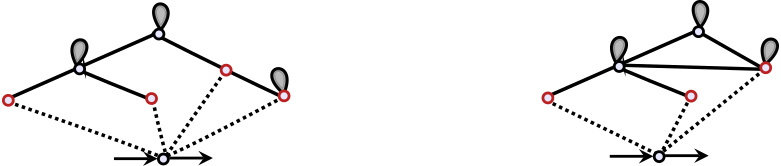
\includegraphics[scale=.35]{tree-like}
%\end{center}
We denote by $\G_\mathsf{s}$, $\G_\mathsf{p}$, $\G_\mathsf{d}$, $\G_\mathsf{t}$, $\G_\mathsf{w}$, $\G_\mathsf{m}$, $\G_\mathsf{\tau}$ and  $\G_\mathsf{u}$ the set of series, parallel, domain, test, word, multiset, tree-like and non-trivial unary graphs.  
%\begin{definition}
%We define \emph{left series-parallel} terms $T_\mathsf{lsp}$, \emph{left parallel} terms $T_\mathsf{lp}$  and \emph{tree-like} terms $T_\tau$ as follows:
%$$\begin{array}{lrlr}
%T_\mathsf{lsp}\qquad\qquad&t, u:=&t\cdot a \cdot b \ \mid\ t \cdot b \ \mid\ t\parallel u \ |\ b&\quad (a\in A_1,\  b\in A_2\cup A_2^\circ).\\
% T_\mathsf{lp}\quad&t:=& u\parallel v&\quad (u,v \in T_\mathsf{lsp}). \\
%T_\tau & t:=&\dom(u\cdot a)& \quad (u\in T_\mathsf{l}).
%\end{array}$$
%We call their graphs respectively \emph{left series-parallel},  \emph{left parallel} and \emph{tree-like} graphs, and denote their set by $\G_\mathsf{lsp}, \G_\mathsf{lp}$ and $\G_{\tau}$ respectively.  
%If $G$ is a tree like graph, we call its \emph{rays} the edges connected to the input. We denote by $R(G)$ the set of letters labeling them.
%\end{definition}
%Tree-like graphs are called so because when we remove their rays, the obtained graph is a tree. Here is an example of a left parallel graph in the left, and a tree-like graph in the right (we did not draw the labels and the orientation of the edges). The rays are the dashed edges. 
%\begin{center}
%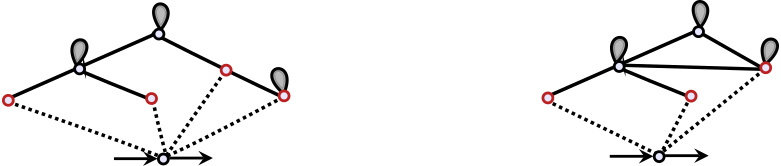
\includegraphics[scale=.4]{tree-like}
%\end{center}
\begin{definition}[Pure components of a pure graph] If $G$ is a pure graph, we can write it as:
$$
\begin{array}{lll}
G=W[ \vec{H}/\vec{x}], &W\in \G_\mathsf{w},\ \vec{H}\subseteq \mathcal{G}_\mathsf{p}\cup\mathcal{G}_{\mathsf{u}}, &     \text{if $G$ is series,}\\
  G=M[\vec{H}/\vec{x}], &M\in \G_\mathsf{m},\  \vec{H}\subseteq \mathcal{G}_\mathsf{s}, & \text{if $G$ is parallel,}\\
   G=M[\vec{H}/\vec{x}], &M\in \G_\mathsf{m},\  \vec{H}\subseteq\mathcal{G}_{\mathsf{d}},& \text{if $G$ is test,} \\
   G=T[\vec{H}/\vec{x}, \vec{M}/\vec{y}], & T\in \G_\tau,\  \vec{H}\subseteq \mathcal{G}_\mathsf{p}\cup \G_\mathsf{u},\  \vec{M}\subseteq \mathcal{G}_\mathsf{m}\cap \G_{\mathsf{p}}\ \text{ and }\ \vec{y}\subseteq R(T), &  \text{if $G$ is domain,} 
\end{array}
$$
where all the substitutions above are guarded.  We call the graphs  $W, M$ and $T$ the \emph{skeleton} of $G$, and the graphs $\vec{H}$ and $\vec{M}$ the \emph{first-layer components} of $G$.  We define the \emph{pure components}  of $G$,  recursively, as  its first-layer components which are pure, together with their pure components. We denote their set $\mathsf{pure}(G)$.
\end{definition}
The first layer components of a pure graph are unique, and the skeleton is unique up to renaming and reorientation of its edges.   
 
%\noindent Below, the skeleton of a series, parallel and test graph, colored in grey.
%\begin{center}
%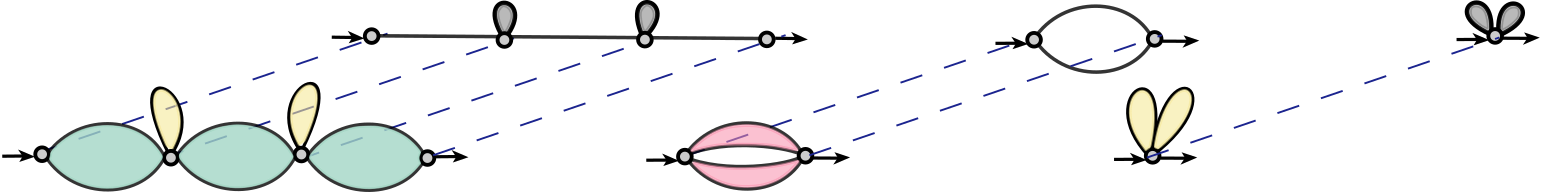
\includegraphics[scale=.35]{skeleton-SPT}
%\end{center}
%The skeleton of a domain graph looks like this.
% \begin{center}
%\includegraphics[scale=.35]{skeleton-D}
%\end{center}
\begin{example} The pure components of the graph $G$ below are  tagged  by the green stars.  At each step of the iteration, we display the skeleton of the graph (linked to the graph by red dashed lines), and the first layer components (linked to the graph by the green dashed lines). 
\begin{center}
\includegraphics[scale=.35]{skeleton-concrete}
\end{center}
\end{example}
\begin{definition}[Pure components of impure graphs]
If $G$ is an impure $\TWT$ graph, we can write it as:
$$
\begin{array}{ll}
G=M[ \vec{H}/\vec{x}], &M\in \G_\mathsf{m},\ \vec{H}\subseteq \mathcal{G}_\mathsf{pure},
\end{array}
$$
where the substitution above is guarded.  The \emph{pure components} of $G$ are the graphs $\vec{H}$ appearing in any such decomposition, which is not unique in general. 
\end{definition}
Note that for impure graphs, the pure components are \emph{not} defined recursively.
% 
%\begin{lemma}\label{lem:no-pure-comp}
%Let $G$ be a graph such that $\mathsf{pure}(G)=\emptyset$.
%If $G$ is series, then it is a word graph. If $G$ is parallel, test or impure, then it is a multiset graph. If $G$ is domain, then it is a tree-like graph. 
%\end{lemma}

%\red{remove from extended abstract.}
%\begin{lemma}\label{lem:pure-substitution}
%Let $G, H$ be pure graphs such that $G[H/x]$ is a guarded substitution. We have: 
%$$\mathsf{pure}(G[H/x])\subseteq  \mathsf{pure}(G)[H/x] \cup \mathsf{pure}(H) \cup \set{H} $$
%\end{lemma}
%\begin{proof}
%We proceed by induction on the structure of $G$. 
%\end{proof}

\subsection{Proof idea of Theorem~\ref{thm:Rec->Reg}}
Here is the general idea of the proof, which follows the same lines as the proof of a similar result for binoids~\cite{Gazdag}. First, we show that if a language is recognizable by an algebra, then it is recognizable by a \emph{type respecting algebra}, that is to say an algebra where we can decompose its domain $D$ into subsets  $D_\mathsf{s}, D_\mathsf{p}$ etc, such that a graph is series,  parallel, etc, if and only if its image by the recognizing homomorphism is in $D_\mathsf{s}$, $D_\mathsf{p}$, etc. 

Let $L$ be a language recognized by homomorphism $h$ and a type respecting algebra $\mathcal{A}$ whose domain is $D$.  For every  $r\in D$,  we show that $L_r$, which is the set of $\TWT$ graphs whose image is $r$, is regular. This is enough to conclude, since $L$ is a union of such languages. 

We associate to every $r\in D$ a new letter $x_r$, and extend $h$ to graphs using these letters by setting $h(x_r)=r$. Let $P\subseteq D$  and $\Sigma$ a subset of the new letters,  we define the language $L^{P,\Sigma}_r$ as the set of graphs whose image by $h$ is $r$, which are allowed to use the new letters from $\Sigma$ and such that the image of their pure components belong to $P$. Our new goal is to show that $L^{P,\Sigma}_r$ is regular. This allows us to conclude that $L_r$ is regular because $L_r=L^{D,\emptyset}_r$.    

To prove that $L^{P,\Sigma}_r$ is regular, we proceed by induction on $P$. Let us discuss the case where $r\in D_\mathsf{s}$, so the graphs of $L^{P,\Sigma}_r$ are series.  When $P$ is empty, these graphs are actually word graphs, and the regularity of this languages is obtained from classical results. For the inductive step, that is, when $P=Q\uplus \set{v}$, we prove the following equality:
$$L^{P,\Sigma}_r=L^{Q,\Sigma\cup\set{x_v}}_r[\mu x_v. L^{Q,\Sigma\cup\set{x_v}}_v/x_v][L^{Q,\Sigma}_v/x_v]  $$
and show that all these substitutions and iterations are guarded. By induction hypothesis, and using the operations of iteration and substitution of the syntax, we conclude that $L^{P,\Sigma}_r$ is regular. 

%\subsection{Type respecting algebra}
%
%\begin{definition}
%Let  $\A$ be an algebra whose domain is $D$. We say that $\A$ is \emph{type respecting} if we can find subsets $D_\mathsf{atomic}$, $D_\mathsf{pure}, D_\mathsf{impure}, D_\mathsf{s}, D_\mathsf{p}, D_\mathsf{d}, D_\mathsf{t}$, $D_\mathsf{lp}$ and $D_\mathsf{\tau}$ of the domain $D$, such that for every term $t$, its graph is pure, impure,  series, parallel, domain, test, left-parallel or tree-like, if and only if the evaluation of $t$ belongs to theses sets respectively.  
%\end{definition}
%
%\begin{lemma}\label{prop:type-respecting-rec}
%If $L$ is a recognizable language of $\TWT$ graphs, then  it is recognizable by a type respecting algebra.
%\end{lemma}
%
%\begin{proof}
%D'abord remarquer que les tree like graphes sont generés par une syntaxe. Et c'est ça qui fait que c'est facile de se rappeler d'eux.
%We need to remember only a finite amount of information to know whether a graph is in each of these sets. 
%\end{proof}
%
%
%
%
%
%\subsection{Proof of Theorem~\ref{thm:Rec->Reg}}
%
%
%
%Let $L$ be a recognizable language. By Prop.~\ref{prop:type-respecting-rec}, we can assume that $L$ is recognized by a type respecting algebra, and keep the same notations used there. Let $h$ be a homomorphism recognizing $L$, and $F\subseteq D$ such that $L=h^{-1}(F)$. We define $L_r$ as the language of graphs whose image (by $h$) is $r$. Our goal is to show that $L_r$ is regular for every $r\in D$. This is enough to conclude because 
%$L=\underset{r\in F}{\bigcup}L_r$.
%\medskip
%
%First, we will show that $L_r$ is regular when \underline{$r\in D_\mathsf{pure}$}. 
%\medskip
%
%  Let $A_\mathsf{pure}$ be a alphabet containing a binary letter for each element of the set $D_\mathsf{s}\cup D_\mathsf{p}$, and a unary letter for each element of  $D_\mathsf{d}\cup D_\mathsf{t}$. If $r\in D_{\mathsf{pure}}$, we denote by $x_r$ its corresponding letter in $A_\mathsf{pure}$. We extend $h$  to terms over  $A\cup A_\mathsf{pure}$, by letting $h(x_r)=r$ for every $r\in D_\mathsf{pure}$.
%\smallskip
%
%Let $P \subseteq  D_{\mathsf{pure}}$, $\Sigma\subseteq A_\mathsf{pure}$ and $r\in D$. We define $L^{P,\Sigma}_r$ as the set of graph terms over the alphabet $A\cup \Sigma$ defined as follows. We let $G\in L^{P,\Sigma}_r$  if and only if:
%\begin{enumerate}
%\item The image of $G$ is $r$.
%\item The image of every pure components of $G$ belongs to $P$.
%\item If $r\in D_\mathsf{s}$,  then $G$ is not a series context for $x_r$.
%\item If $r\in D_\mathsf{p}\cup D_\mathsf{t}$,  then $G$ is not a parallel context for $x_r$.
%\end{enumerate}
%
%
%\noindent We show, by induction on the size of $P$, that $L^{P, \Sigma}_s$ is regular  if  the letters associated to $P$ and the set $\Sigma$ are disjoint. We start by the inductive step.
%\smallskip
%
% \noindent \textbf{Inductive step.} Suppose that $P=Q\uplus \set{v}$. We prove the following equality:
%$$L^{P,\Sigma}_r=L^{Q,\Sigma\cup\set{x_v}}_r[\mu x_v. L^{Q,\Sigma\cup\set{x_v}}_v/x_v][L^{Q,\Sigma}_v/x_v] \qquad\qquad(\star) $$
%Substitutions and iterations in $(\star)$ are guarded thanks to the conditions 3 and 4 above. 
%Using this equality and the induction hypothesis, we can conclude that the language $L^{P,\Sigma}_r$ is regular. 
%
%
%The right-to-left implication follows from Lem.~\ref{lem:pure-substitution}.  Let us show the other inclusion. 
%
%\noindent A \emph{$v$-component} of a graph is a pure component of this graph whose image by $h$ is $v$.  The \emph{$v$-reduct} of a graph is the graph obtained by replacing every $v$-component by the letter $x_v$, such that the resulting graph has no $v$-components.  Let $G$ be a graph in  $L^{P,\Sigma}_r$,  we let: 
%\begin{itemize}
%\item $H$ be the $v$-reduct of $G$,
%\item $S$ be the set of $v$-reducts of the $v$-components of $G$.
%\item $T$ be the set of $v$-components of $G$, which do not contain further $v$-components.
%\end{itemize}
%We have the following inclusions: 
%$$G\in H[\mu x_r. T/x_r][S/x_r],\quad H\subseteq L^{Q,\Sigma\cup\set{x_v}}_r,\quad S\subseteq L^{Q,\Sigma\cup\set{x_v}}_v\ \  \text{ and }\ \ T\subseteq L^{Q,\Sigma}_v.$$
%This concludes the left-to-right inclusion of $(\star)$, and  the inductive step. Now let us treat the base case.  We have two base cases, one of them will make a call to the inductive step. 
%\medskip
%
%
% \noindent \textbf{Base case 1.} $P$ is empty and $r\in D_\mathsf{s}\cup D_\mathsf{p}\cup D_\mathsf{t}$. Then the graphs of $L^{\emptyset,\Sigma}_r$ are either word graphs or multiset graphs. Their regularity follow from the case of words and commutative words.
%\medskip
%
%\begin{observation}
%Using base case 1 and the inductive step, we have that 
%$L^{P,\Sigma}_r$ is regular if $r\in D_\mathsf{s}\cup D_\mathsf{p}\cup D_\mathsf{t}$ and $P\subseteq D_\mathsf{s}\cup D_\mathsf{p}\cup D_\mathsf{t}$. 
%\end{observation}
%\medskip
%
%\noindent \textbf{Base case 2.} $P$ is empty and $r\in D_\mathsf{d}$.  The graphs of $L^{\emptyset,\Sigma}_r$ are tree-like graphs. 
%Let $S$ be the set of pairs $(v,a)$ such that $v\in D_{\mathsf{lp}}$, $a\in A_1$ and $r=\dom(v\cdot a)$. We have that:
%$$ L^{\emptyset, \Sigma}_r=\underset{(v,a)\in S}{\bigcup}\dom\big({L^{D_\mathsf{s}\cup D_\mathsf{t},\Sigma}_v\cdot a}\big)$$
%because left parallel graphs do not have unary pure components. The set $ L^{\emptyset, \Sigma}_r$ is regular thanks to the observation above. 
%\medskip
%
%When $r\in D_\mathsf{atomic}$,  $L_r$ is regular because it is finite. 
%\medskip
%
%Let us show that $L_r$ is regular when $r\in D_\mathsf{impure}$.
%Note that
%$$L_r= L^{\emptyset, A_\mathsf{pure}}_r[L_v/x_v, v\in D_\mathsf{pure}]$$
%The language $L^{\emptyset, A_\mathsf{pure}}_r$ is a language of multiset graphs, it regularity follows from the case of commutative words. The languages $L_v$ are regular because $v$ is pure, and this case was treated above. This concludes the proof. 